%%%%%%%%%%%%%%%%%%%%%%%%%%%%%%%%%%%%%%%%%%%%%%%%%%%%%%%%%%%%%%%%%%%%%%%%%%%

\documentclass{standalone}

\usepackage{mathptmx}
\usepackage{tikz}
\usetikzlibrary{external}
\tikzexternalize{number-line}

%% We default to Times.
\renewcommand{\rmdefault}{ptm}
\renewcommand{\ttdefault}{pcr}
%% Enable Times/Palatino main text font.
\normalfont\selectfont

%% A tick on the x-axis.
%%
%% #1 -- A point on the x-axis.
\newcommand{\tick}[1]{%%
  \draw[tickStyle] (#1,\ylow+\tickdx) -- (#1,\ylow-\tickdx);
  \node at (#1,\ylow-\tickdx) [below] {$#1$};
}

%% The x-axis.
\newcommand{\xAxis}{%%
  \draw[axisStyle] (-1.5,0) -- (4.5,0);
  \foreach \x in {-1,0,1,2,3,4}{
    \tick{\x}
  };
}

%% A point on the x-axis.
%%
%% #1 -- The x-coordinate of the point.
%% #2 -- Label the point with this name.
\newcommand{\xPoint}[2]{%%
  \node[nodeStyle] at (#1,\ylow) {};
  \node at (#1,\ylow+\tickdx) [above] {$#2$};
}

%% A real number as a point on the number line.

\begin{document}

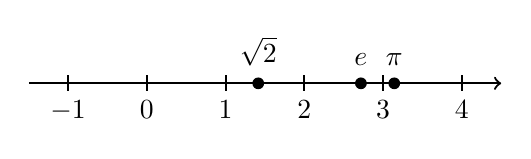
\begin{tikzpicture}[%%
  axisStyle/.style={->,thick},%%
  nodeStyle/.style={circle,inner sep=1.5pt,fill=black,black},%%
  tickStyle/.style={-,thick}
]
%%
%%
\pgfmathsetmacro{\tickdx}{0.1}
\pgfmathsetmacro{\ylow}{0}
%%
%% The number line.
\xAxis
%% Some points on the line.
\xPoint{1.41421356237310}{\sqrt{2}}
\xPoint{2.71828182845905}{e}
\xPoint{3.14159265358979}{\pi}
\end{tikzpicture}

\end{document}
